\documentclass[runningheads]{llncs}
\usepackage[T1]{fontenc}
\usepackage{graphicx}

\begin{document}
\title{TLA+}
\author{Anna Aimeri, Sebastián Giraudo, Valentín Negrelli}
\institute{Facultad de Matemática, Astronomía, Física y Computación, Av. Medina Allende s/n, Córdoba, Argentina}
\maketitle              % typeset the header of the contribution
%
\begin{abstract}
The abstract should briefly summarize the contents of the paper in
150--250 words.

\keywords{First keyword  \and Second keyword \and Another keyword.}
\end{abstract}

\section{Contexto de creación}

\section{Objetivo}
TLA+ es un lenguaje de especificación formal multi-propósito particularmente útil para describir sistemas distribuidos y concurrentes. Se trata de un lenguaje declarativo, jerárquico, y escalable a especificaciones de grandes sistemas, que provee una abstracción consistente sobre varios verificadores como backend. 
Las propiedades que TLA+ puede chequear son condiciones sobre ejecuciones individuales. Además permite verificar invariantes sobre comportamientos válidos tales como fairness y algunas propiedades de lógica temporal básica que respondan a características de safety y liveness.
Como el objetivo es especificar propiedades sobre las variables libres del modelo, es útil en la etapa de arquitectura y diseño del software, una vez que se cuenta con la especificación y antes de codificar la implementación. A su vez, es posible apoyarse en la herramienta para derivar casos de tests, dado que un diseño certero del modelo nos provee el conjunto de propiedades a verificar para nuestra implementación.

\section{Descripción del lado del usuario}

\section{Aspectos técnicos}

\section{Casos de estudio}


Subsequent paragraphs, however, are indented.

\paragraph{Sample Heading (Fourth Level)}
The contribution should contain no more than four levels of
headings. Table~\ref{tab1} gives a summary of all heading levels.


\noindent Displayed equations are centered and set on a separate
line.
\begin{equation}
x + y = z
\end{equation}
Please try to avoid rasterized images for line-art diagrams and
schemas. Whenever possible, use vector graphics instead (see
Fig.~\ref{fig1}).

\begin{figure}
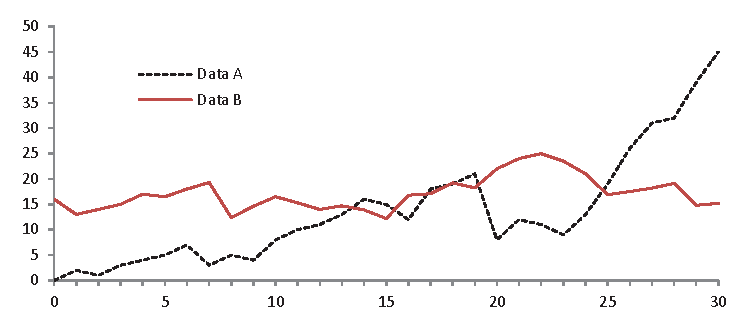
\includegraphics[width=\textwidth]{fig1.eps}
\caption{A figure caption is always placed below the illustration.
Please note that short captions are centered, while long ones are
justified by the macro package automatically.} \label{fig1}
\end{figure}

\begin{theorem}
This is a sample theorem. The run-in heading is set in bold, while
the following text appears in italics. Definitions, lemmas,
propositions, and corollaries are styled the same way.
\end{theorem}

For citations of references, we prefer the use of square brackets
and consecutive numbers. Citations using labels or the author/year
convention are also acceptable. The following bibliography provides
a sample reference list with entries for journal
articles~\cite{ref_article1}, an LNCS chapter~\cite{ref_lncs1}, a
book~\cite{ref_book1}, proceedings without editors~\cite{ref_proc1},
and a homepage. Multiple citations are grouped
\cite{ref_article1,ref_lncs1,ref_book1},
\cite{ref_article1,ref_book1,ref_proc1}.

\begin{credits}
\subsubsection{\ackname} A bold run-in heading in small font size at the end of the paper is
used for general acknowledgments, for example: This study was funded
by X (grant number Y).

\subsubsection{\discintname}
It is now necessary to declare any competing interests or to specifically
state that the authors have no competing interests. Please place the
statement with a bold run-in heading in small font size beneath the
(optional) acknowledgments\footnote{If EquinOCS, our proceedings submission
system, is used, then the disclaimer can be provided directly in the system.},
for example: The authors have no competing interests to declare that are
relevant to the content of this article. Or: Author A has received research
grants from Company W. Author B has received a speaker honorarium from
Company X and owns stock in Company Y. Author C is a member of committee Z.
\end{credits}
%
% ---- Bibliography ----
%
% BibTeX users should specify bibliography style 'splncs04'.
% References will then be sorted and formatted in the correct style.
%
% \bibliographystyle{splncs04}
% \bibliography{mybibliography}
%
\begin{thebibliography}{8}
\bibitem{ref_article1}
Author, F.: Article title. Journal \textbf{2}(5), 99--110 (2016)

\bibitem{ref_lncs1}
Author, F., Author, S.: Title of a proceedings paper. In: Editor,
F., Editor, S. (eds.) CONFERENCE 2016, LNCS, vol. 9999, pp. 1--13.
Springer, Heidelberg (2016). \doi{10.10007/1234567890}

\bibitem{ref_book1}
Author, F., Author, S., Author, T.: Book title. 2nd edn. Publisher,
Location (1999)

\bibitem{ref_proc1}
Author, A.-B.: Contribution title. In: 9th International Proceedings
on Proceedings, pp. 1--2. Publisher, Location (2010)

\end{thebibliography}
\end{document}
